\documentclass[UTF8,11pt]{ctexart}
\usepackage[a4paper,margin=22mm]{geometry}
\usepackage{amsmath,amssymb,bm,graphicx,adjustbox,fvextra,longtable,array}
\xeCJKDeclareCharClass{CJK}{"2160 -> "217F, "2460 -> "249B, "2200 -> "22FF}
\newcommand{\fitmath}[1]{\begin{adjustbox}{max width=\linewidth}$\displaystyle #1$\end{adjustbox}}
\setlength{\parindent}{0pt}\setlength{\parskip}{.65em}\renewcommand{\arraystretch}{1.3}
\sloppy\allowdisplaybreaks
\begin{document}
\section*{2020 年计算机统考 408 · 答案与解析}
\subsection*{2020 全国硕士研究生招生考试 计算机学科专业基础试题参考答案}

\subsection*{一、单项选择题}

\begin{center}\begin{adjustbox}{max width=\linewidth}\begin{tabular}{|c|c|c|c|c|c|c|c|c|c|c|c|c|c|c|c|}\hline
1 & C & 2 & D & 3 & A & 4 & C & 5 & B & 6 & B & 7 & A & 8 & B\\\hline
9 & C & 10 & B & 11 & A & 12 & B & 13 & A & 14 & D & 15 & D & 16 & A\\\hline
17 & B & 18 & A & 19 & C & 20 & C & 21 & B & 22 & C & 23 & B & 24 & A\\\hline
25 & D & 26 & D & 27 & B & 28 & D & 29 & B & 30 & D & 31 & B & 32 & C\\\hline
33 & C & 34 & B & 35 & C & 36 & D & 37 & A & 38 & D & 39 & C & 40 & D\\\hline\end{tabular}\end{adjustbox}\end{center}

1. 【解析】上三角矩阵按列优先存储，先存储仅 1 个元素的第一列，再存储有 2 个元素的第二列，以此类推。\(\displaystyle m_{7,\allowbreak 2}\) 位于左下角，对应右上角的元素为 \(\displaystyle m_{2,\allowbreak 7}\)，在 \(\displaystyle m_{2,\allowbreak 7}\) 之前存有：第 1 列 1 个，第 2 列 2 个，……第 6 列 6 个，第 7 列 1 个。前面共存有 \(\displaystyle 1+2+3+4+5+6+1=22\) 个元素（数组下标范围为 0～21），注意数组下标从 0 开始，故 \(\displaystyle m_{2,\allowbreak 7}\) 在数组 N 中的下标为 22，即 \(\displaystyle m_{7,\allowbreak 2}\) 在数组 N 中的下标为 22。


2. 【解析】按题意，出入栈操作的过程如下：


\begin{center}\begin{adjustbox}{max width=\linewidth}\begin{tabular}{|>{\raggedright\arraybackslash}p{\dimexpr(\linewidth-6\tabcolsep-4\arrayrulewidth)/3\relax}|>{\raggedright\arraybackslash}p{\dimexpr(\linewidth-6\tabcolsep-4\arrayrulewidth)/3\relax}|>{\raggedright\arraybackslash}p{\dimexpr(\linewidth-6\tabcolsep-4\arrayrulewidth)/3\relax}|}\hline
操作 & 栈内元素 & 出栈元素\\\hline
Push & a & \\\hline
Push & a b & \\\hline
Pop & a & b\\\hline
Push & a c & \\\hline
Pop & a & c\\\hline
Push & a d & \\\hline
Push & a d e & \\\hline
Pop & a d & e\\\hline\end{tabular}\end{adjustbox}\end{center}

故出栈序列为 b，c，e。


3. 【解析】二叉树采用顺序存储时，用数组下标来表示结点之间的父子关系。对于一棵高度为 5 的二


叉树，为了满足任意性，其 1～5 层的所有结点都要被存储起来，即考虑为一棵高度为 5 的满二叉树，总共需要存储单元的数量为 1+2+4+8+16 = 31。


4. 【解析】森林 F 的先根遍历序列对应其二叉树 T 的先序遍历序列，森林 F 的中根遍历序列对应其二叉树 T 的中序遍历序列。即 T 的先序遍历序列为 a，b，c，d，e，f，中序遍历序列为 b，a，d，f，e，c。根据二叉树 T 的先序序列和中序序列可以唯一确定它的结构，构造过程如下：


\begin{center}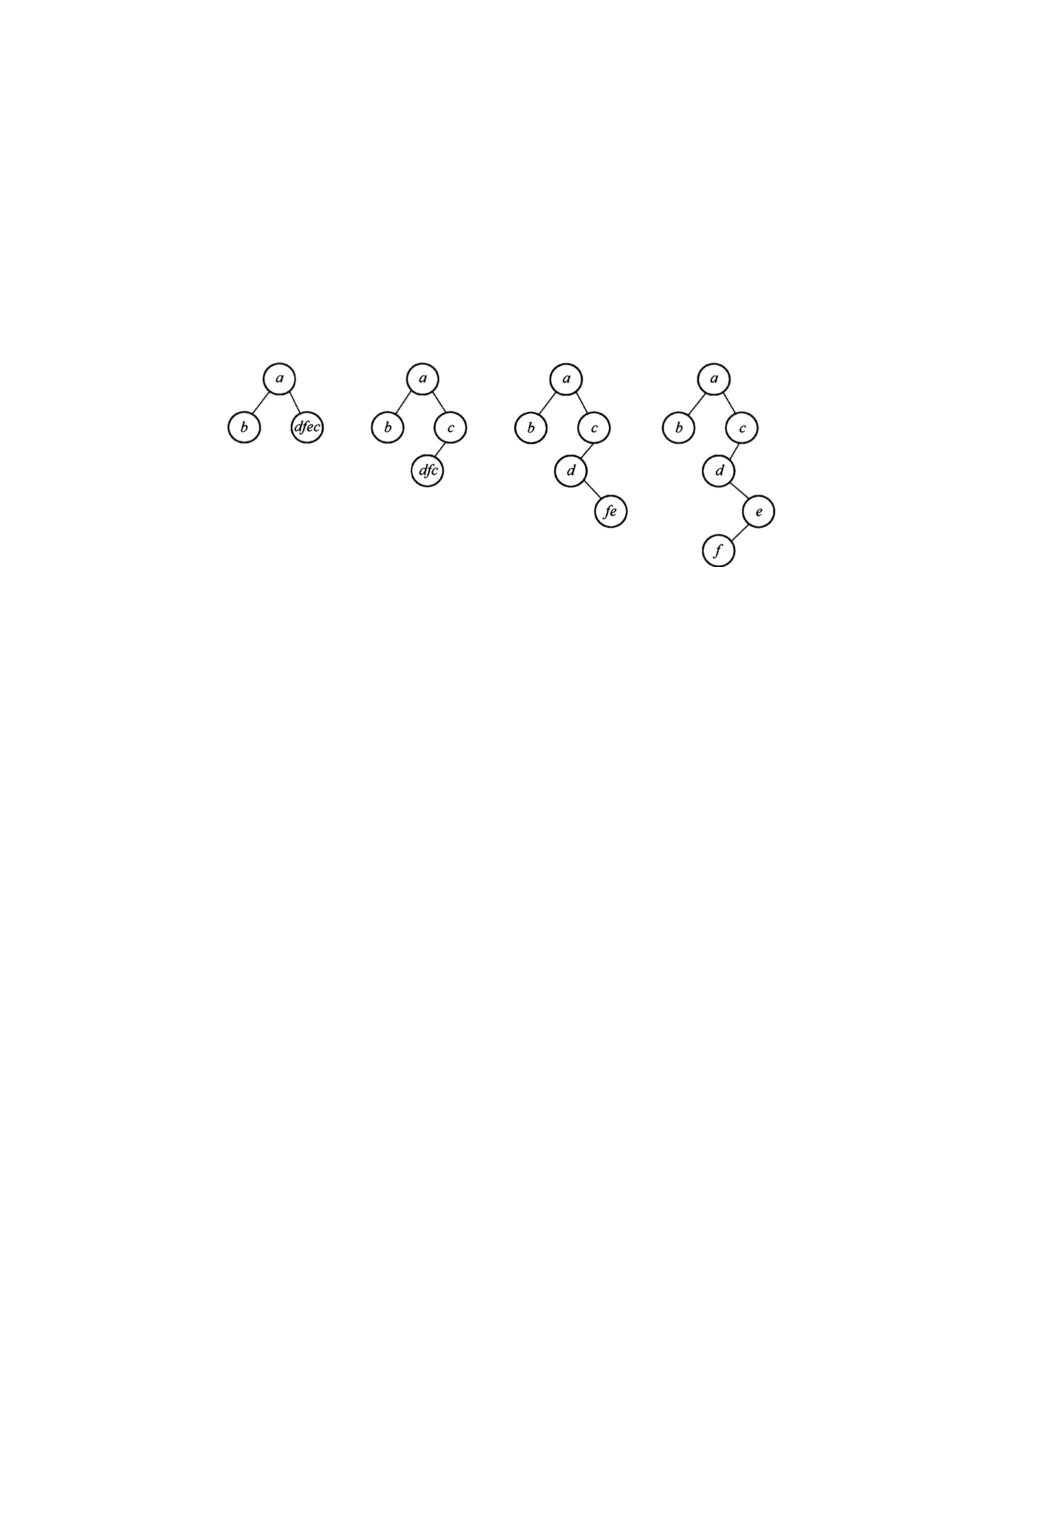
\includegraphics[width=.65\linewidth,height=.4\textheight,keepaspectratio]{../assets/figures/2020-answers-p002-b002.pdf}\end{center}

可以得到二叉树 T 的后序序列为 b，f，e，d，c，a。


5. 【解析】每个选项都逐一验证，选项 B 生成二叉排序树的过程如下：


\begin{center}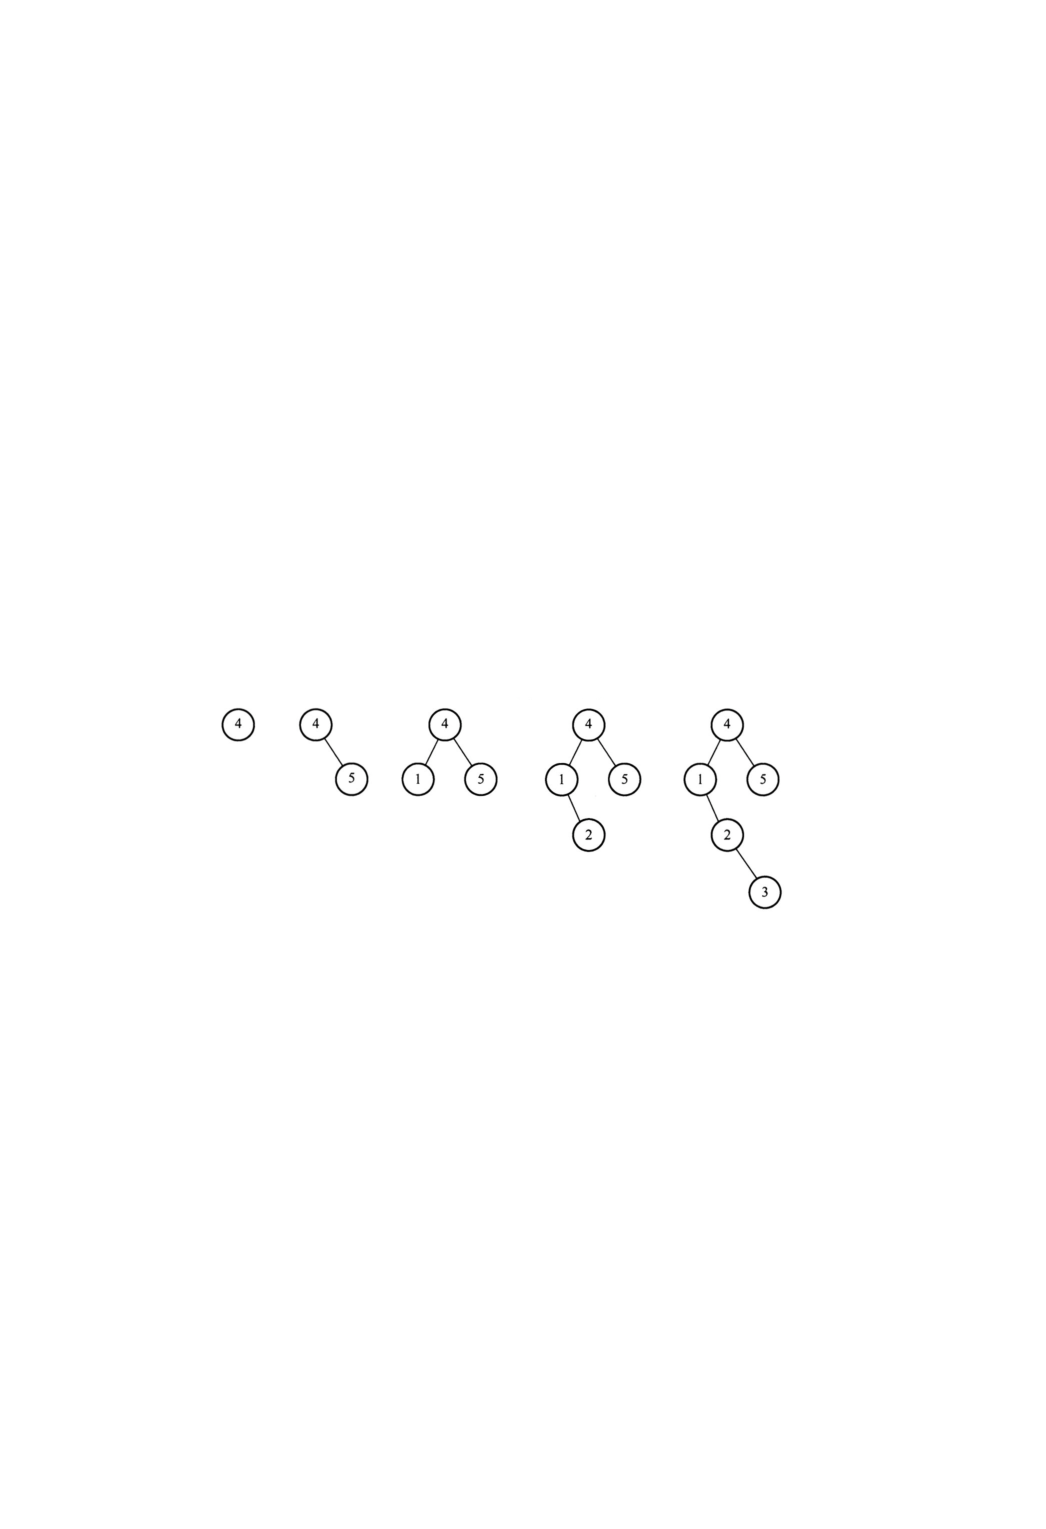
\includegraphics[width=.65\linewidth,height=.4\textheight,keepaspectratio]{../assets/figures/2020-answers-p002-b005.pdf}\end{center}

显然选项 B 错误。


6. 【解析】DFS 是一个递归算法，在遍历过程中，先访问的顶点被压入栈底。设在图中有顶点 \(\displaystyle v_i\)，它有后继顶点 \(\displaystyle v_j\)，即存在边 \(\displaystyle \langle v_i,\allowbreak v_j\rangle\)。根据 DFS 的规则，\(\displaystyle v_i\) 入栈后，必先遍历完其后继顶点后 \(\displaystyle v_i\) 才会出栈，也就是说 \(\displaystyle v_i\) 会在 \(\displaystyle v_j\) 之后出栈，在如题所指的过程中，\(\displaystyle v_i\) 在 \(\displaystyle v_j\) 后打印。由于 \(\displaystyle v_i\) 和 \(\displaystyle v_j\) 具有任意性，从上面的规律可以看出，输出顶点的序列是逆拓扑有序序列。


7. 【解析】Kruskal 算法：按权值递增顺序依次选取 \(\displaystyle n-1\) 条边，并保证这 \(\displaystyle n-1\) 条边不构成回路。初始构造一个仅含 \(\displaystyle n\) 个顶点的森林；第一步，选取权值最小的边 \(\displaystyle (b,\allowbreak f)\) 加入最小生成树；第二步，剩余边中权值最小的边为 \(\displaystyle (b,\allowbreak d)\)，加入最小生成树，第二步操作后权值最小的边 \(\displaystyle (d,\allowbreak f)\) 不能选，因为会与之前已选取的边形成回路；接下来依次选取权值 9、10、11 对应的边加入最小生成树，此时 6 个顶点形成了一棵树，最小生成树构造完成。按照上述过程，加到最小生成树的边依次为 \(\displaystyle (b,\allowbreak f),\allowbreak (b,\allowbreak d),\allowbreak (a,\allowbreak e),\allowbreak (c,\allowbreak e),\allowbreak (b,\allowbreak e)\)。其生成过程如下所示。


\begin{center}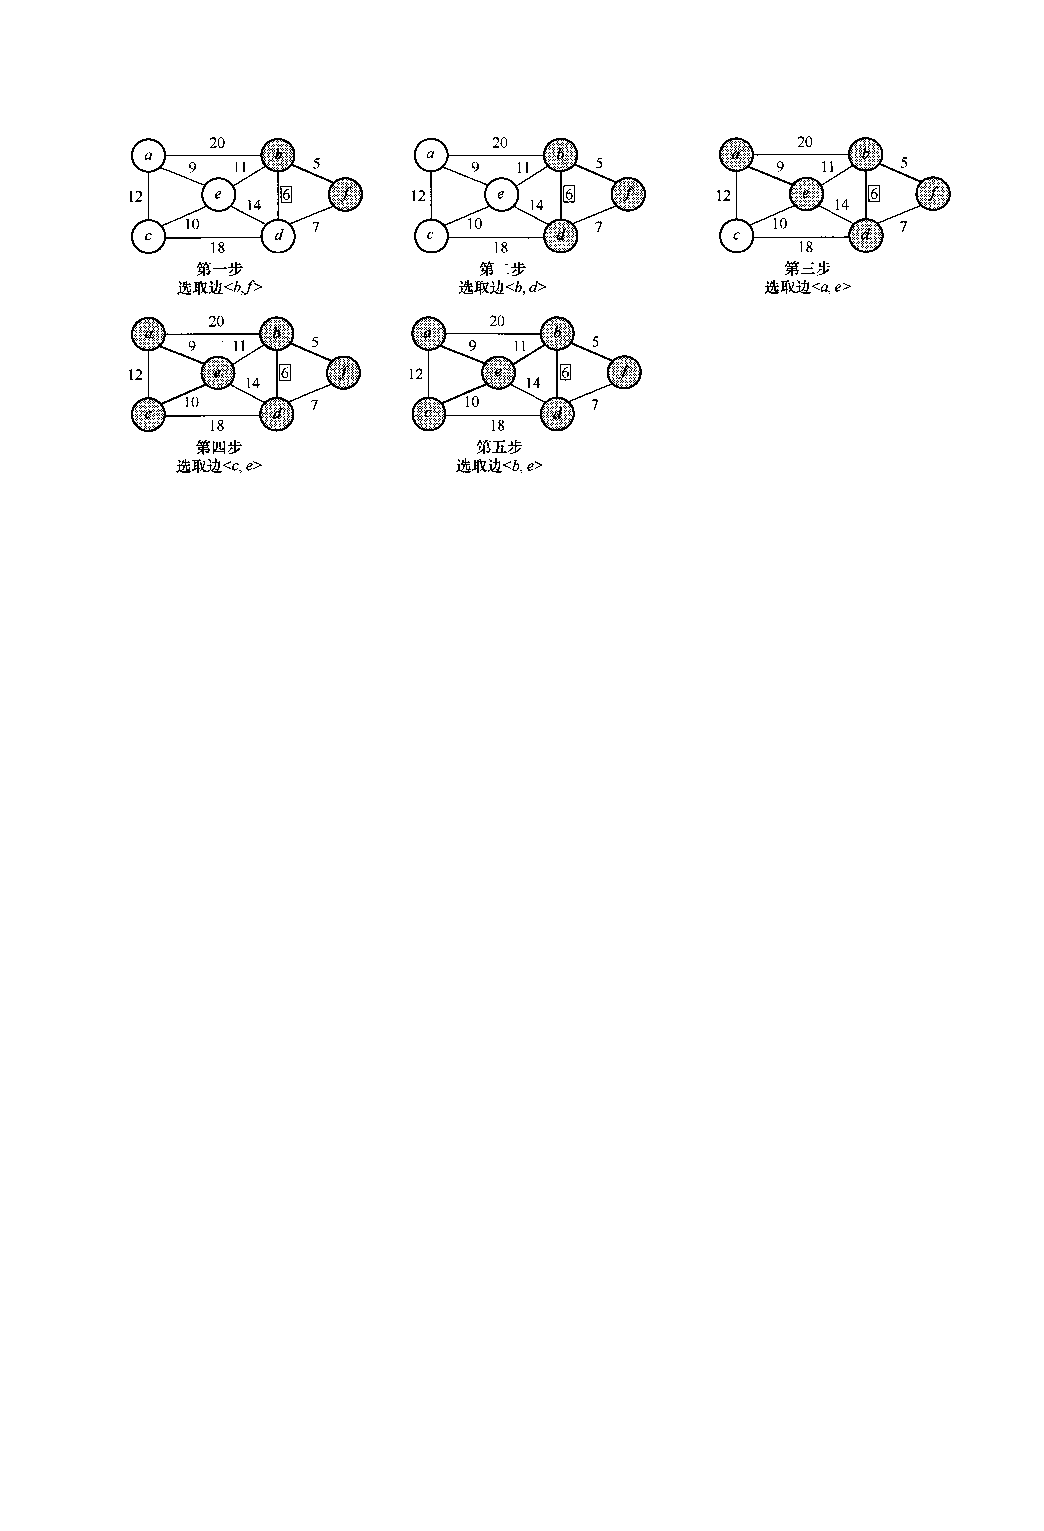
\includegraphics[width=.65\linewidth,height=.4\textheight,keepaspectratio]{../assets/figures/2020-answers-p003-b000.pdf}\end{center}

8. 【解析】关键路径是指权值之和最大而非边数最多的路径，故选项A错误。选项B 正确，是关键路径的概念。无论是存在一条还是存在多条关键路径，增加任一关键活动的时间都会延长工程的工期，因为关键路径始终是权值之和最大的那条路径，选项C错误。仅有一条关键路径时，减少关键活动的时间会缩短工程的工期：存在多条关键路径时，缩短一条关键活动的时间不一定会缩短工程的工期，缩短了路径长度的那条关键路径不一定还是关键路径，选项D错误。


9. 【解析】这是一道简单的概念题。堆是一棵完全树，采用一维数组存储，故\(\displaystyle \mathrm{I}\)正确，\(\displaystyle \mathrm{II}\)正确。大根堆只要求根结点值大于左右孩子值，并不要求左右孩子值有序，\(\displaystyle \mathrm{III}\)错误。堆的定义是递归的，所以其左右子树也是大根堆，所以堆的次大值一定是其左孩子或右孩子，\(\displaystyle \mathrm{IV}\)正确。


10. 【解析】一个 4 阶 B 树的任意非叶结点至多含有 \(\displaystyle m-1=3\) 个关键字，在关键字依次插入的过程中，会导致结点不断分裂，插入过程如下所示。


\begin{center}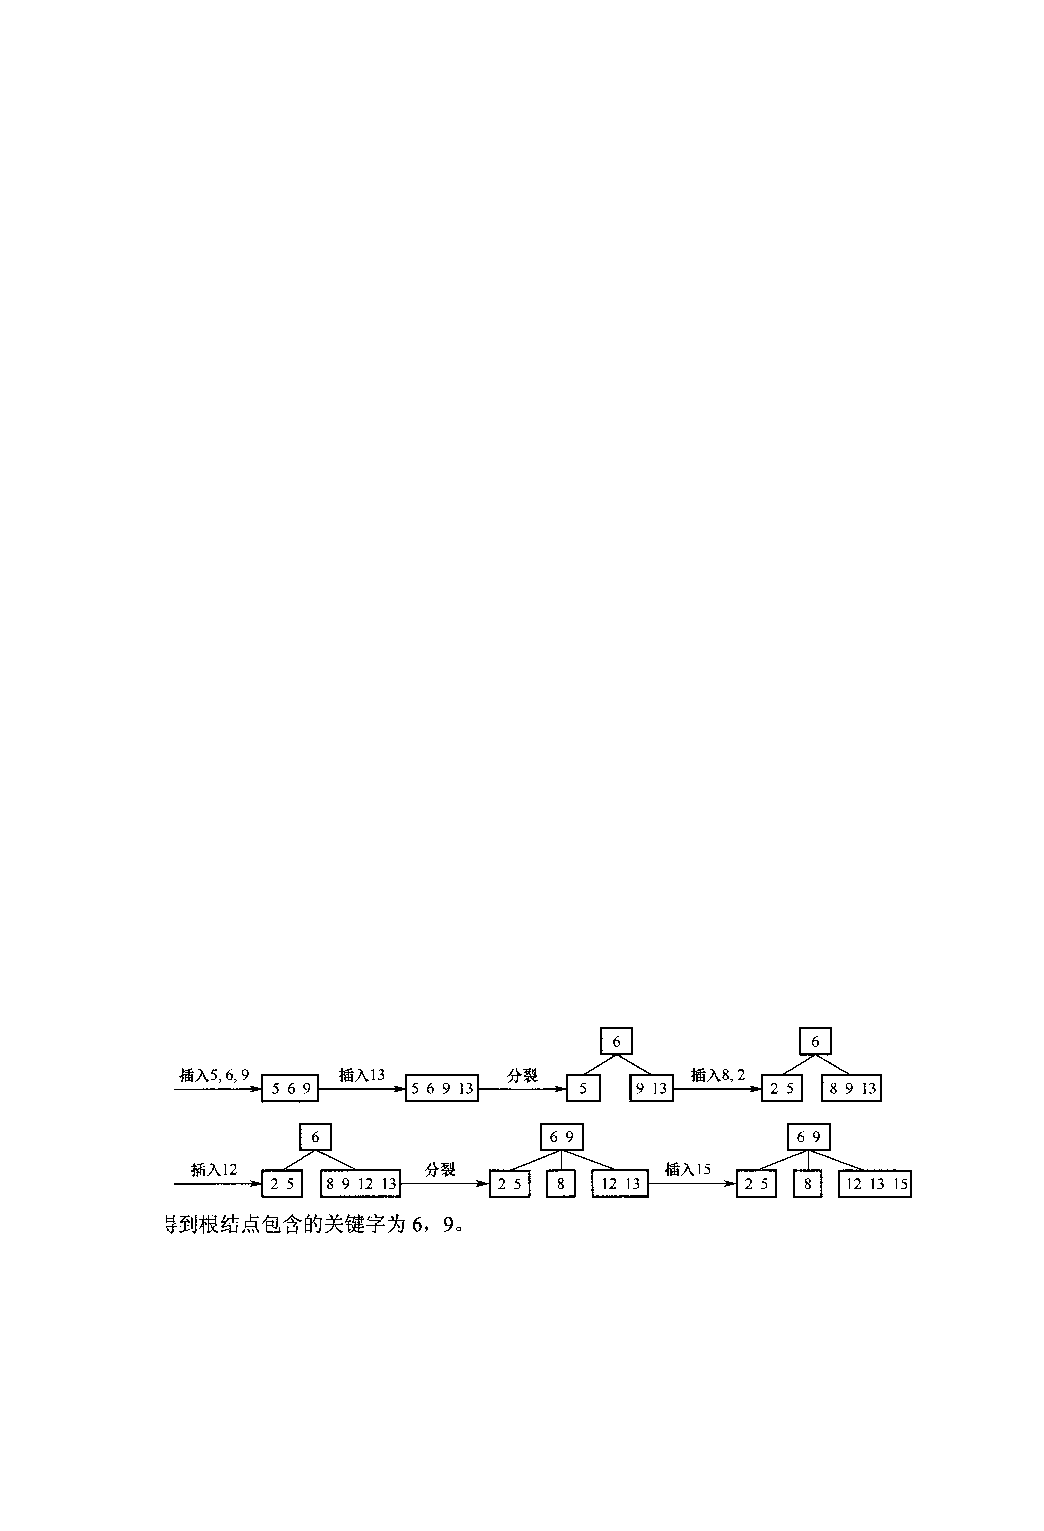
\includegraphics[width=.65\linewidth,height=.4\textheight,keepaspectratio]{../assets/figures/2020-answers-p003-b004.pdf}\end{center}

得到根结点包含的关键字为 6，9。


11. 【解析】考虑较极端的情况，对于有序数组，直接插入排序的比较次数为 \(\displaystyle n-1\)，简单选择排序的比较次数始终为 \(\displaystyle 1+2+\cdots+n-1=n(n-1)/2\)，\(\displaystyle \mathrm{I}\) 正确。两种排序方法的辅助空间都是 \(\displaystyle O(1)\)，无差别，\(\displaystyle \mathrm{II}\) 错误。初始有序时，移动次数均为 0；对于通常情况，直接插入排序每趟插入都


需要依次向后挪位，而简单选择排序只需与找到的最小元素交换位置，后者的移动次数少很多，\(\displaystyle \mathrm{III}\) 错误。


12. 【解析】机器字长是指 CPU 内部用于整数运算数据通路的宽度。CPU 内部数据通路是指 CPU 内部的数据流经路径及路径上的部件，主要是CPU 内部进行数据运算、存储和传送部件，这些部件宽度基本上要一致才能相互匹配。因此，机器字长等于CPU 内部用于整数运算的运算器位数和通用寄存器宽度。


13. 【解析】\(\displaystyle \mathrm{C800\,0000H}=1100\,1000\,0000\,0000\,0000\,0000\,0000\,0000_2\)。将其转换为对应的 float 型或 int 型：\textcircled{1} 为 float 型时，尾数隐藏最高位 1，数符为 1 表示负数，阶码 \(\displaystyle 1001\,0000_2=2^7+2^4=128+16\)，再减去偏置值 127 得到 17，算出 \(\displaystyle x=-2^{17}\)。\textcircled{2} 为 int 型时，带符号补码，为负数，数值部分取反加 1，得 0111 1000 0000 0000 0000 0000 0000 0000，算出 \(\displaystyle x=-7\times2^{27}\)。


14. 【解析】在 32 位计算机中，按字节编址，根据小端方式和按边界对齐的定义，给出变量 a 的存放方式如下：


\begin{center}\begin{adjustbox}{max width=\linewidth}\begin{tabular}{|>{\raggedright\arraybackslash}p{\dimexpr(\linewidth-10\tabcolsep-6\arrayrulewidth)/5\relax}|>{\raggedright\arraybackslash}p{\dimexpr(\linewidth-10\tabcolsep-6\arrayrulewidth)/5\relax}|>{\raggedright\arraybackslash}p{\dimexpr(\linewidth-10\tabcolsep-6\arrayrulewidth)/5\relax}|>{\raggedright\arraybackslash}p{\dimexpr(\linewidth-10\tabcolsep-6\arrayrulewidth)/5\relax}|>{\raggedright\arraybackslash}p{\dimexpr(\linewidth-10\tabcolsep-6\arrayrulewidth)/5\relax}|}\hline
地址 & 2020 FE00H & 2020 FE01H & 2020 FE02H & 2020 FE03H\\\hline
数值 & 未知 & 未知 &  & \\\hline
说明 & x1（LSB） & x1（MSB） &  & \\\hline\end{tabular}\end{adjustbox}\end{center}

\begin{center}\begin{adjustbox}{max width=\linewidth}\begin{tabular}{|>{\raggedright\arraybackslash}p{\dimexpr(\linewidth-10\tabcolsep-6\arrayrulewidth)/5\relax}|>{\raggedright\arraybackslash}p{\dimexpr(\linewidth-10\tabcolsep-6\arrayrulewidth)/5\relax}|>{\raggedright\arraybackslash}p{\dimexpr(\linewidth-10\tabcolsep-6\arrayrulewidth)/5\relax}|>{\raggedright\arraybackslash}p{\dimexpr(\linewidth-10\tabcolsep-6\arrayrulewidth)/5\relax}|>{\raggedright\arraybackslash}p{\dimexpr(\linewidth-10\tabcolsep-6\arrayrulewidth)/5\relax}|}\hline
地址 & 2020 FE04H & 2020 FE05H & 2020 FE06H & 2020 FE07H\\\hline
数值 & 00H & 00H & 34H & 12H\\\hline
说明 & x2（LSB） &  &  & x2（MSB）\\\hline\end{tabular}\end{adjustbox}\end{center}

于是，34H 所在存储单元的地址为 2020 FE06H。


15. 【解析】Cache 由 SRAM组成：TLB 通常由相联存储器组成，也可由 SRAM组成。DRAM 需要不断刷新，性能偏低，不适合组成 TLB 和 Cache。选项A、B和C都是 TLB和 Cache特点。


16. 【解析】48 条指令需要 6 位操作码字段 \(\displaystyle (2^5<48<2^6)\)，4 种寻址方式需要 2 位寻址特征位 \(\displaystyle (4=2^2)\)，还剩 \(\displaystyle 16-6-2=8\) 位作为地址码，故直接寻址范围为 0～255。注意，主存地址不能为负。


17. 【解析】CPI 表示执行指令所需的时钟周期数。对于一个程序或一台机器来说，其 CPI 指执行该程序或机器指令集中的所有指令所需的平均时钟周期数。对于单周期 CPU，令指令周期 = 时钟周期，CPI = 1，\(\displaystyle \mathrm{I}\) 正确。对于多周期 CPU，CPU 的执行过程分成几个阶段，每个阶段用一个时钟去完成，每种指令所用的时钟数可以不同，CPI > 1，\(\displaystyle \mathrm{II}\) 错误。对于基本流水线 CPU，让每个时钟周期流出一条指令，CPI = 1，\(\displaystyle \mathrm{III}\) 正确。超标量流水线 CPU 在每个时钟周期内


并发执行多条独立的指令，每个时钟周期流出多条指令，CPI < 1，\(\displaystyle \mathrm{IV}\) 错误。


18. 【解析】自陷是一种内部异常，A错误。在80x86中，用于程序调试的“断点设置”功能是通过“自陷”方式实现的，选项B 正确。执行到自陷指令时，无条件或有条件地自动调出操作系统内核程序进行执行，选项C正确。CPU 执行“陷阱指令”后，会自动地根据不同“陷阱”类型进行相应的处理，然后返回到“陷阱指令”的下一条指令执行，选项D正确。


19. 【解析】每个时钟周期传送 2 次，故每秒传送的次数 = 时钟频率\(\displaystyle \times\)2 = 2.4G\(\displaystyle \times\)2/s。总线带宽 = 每秒传送次数\(\displaystyle \times\)2B\(\displaystyle \times\)2 = 2.4G\(\displaystyle \times\)2\(\displaystyle \times\)2B\(\displaystyle \times\)2/s = 19.2GB/s。题中已给出总线带宽公式，降低了难度。公式中的“\(\displaystyle \times\)2B”是因为每次传输 16 位数据，“\(\displaystyle \times\)2”是因为采用点对点全双工总线，两个方向可同时传输信息。


20. 【解析】访存时缺页属于内部异常，\(\displaystyle \mathrm{I}\) 错误；定时器到时描述的是时钟中断，属于外部中断，\(\displaystyle \mathrm{II}\) 正确；网络数据包到达描述的是 CPU 执行指令以外的事件，属于外部中断，\(\displaystyle \mathrm{III}\) 正确。


21. 【解析】由CPU内部产生异常称为内中断，内中断都是不可屏蔽中断。通过中断请求线 INTR和NMI，从CPU外部发出的中断请求为外中断，通过 INTR信号线发出的外中断是可屏蔽中断，而通过 NMI信号线发出的是不可屏蔽中断。不可屏蔽中断不受中断标志位的影响，即使在关中断的情况下也会被响应，选项 A 正确。不可屏蔽中断的处理优先级最高，任何时候只要发生不可屏蔽中断，都要中止现行程序的执行，转到不可屏蔽中断处理程序执行，选项C正确。CPU 响应中断需要满足3个条件：\textcircled{1} 中断源有中断请求：\textcircled{2} CPU 允许中断及开中断：\textcircled{3} 一条指令执行完毕，且没有更紧迫的任务。故选项B错误。


22. 【解析】周期挪用法由 DMA 控制器挪用一个或几个主存周期来访问主存，传送完一个数据字后立即释放总线，是一种单字传送方式，每个字传送完后 CPU 可以访问主存，选项C 错误。停止CPU 访存法则是指在整个数据块传送过程中，使CPU脱离总线，停止访问主存。


23. 【解析】多个进程可同时以“读”或“写”方式打开文件，操作系统并不保证写操作的互斥性，进程可通过系统调用对文件加锁，保证互斥写（读者-写者问题），选项 A错误。整个系统只有一个系统打开文件表，同一个文件打开多次只需改变引用计数，选项B正确。用户进程的打开文件表关于同一个文件不一定相同，例如读写指针位置不一定相同，选项C错误。进程关闭文件时，文件的引用计数减1，引用计数变为0 时才删除系统打开文件表中的表项，选项D错误。


24. 【解析】索引分配支持变长的文件，同时可以随机访问文件的指定数据块，选项 A正确。链接分配不支持随机访问，需要依靠指针依次访问，选项B错误。连续分配的文件长度固定，不支持


可变文件长度（连续分配的文件长度虽然也可变，但是需大量移动数据，代价较大，相比之下不太合适），选项 C错误。动态分区分配是内存管理方式，不是磁盘空间的管理方式，选项D错误。


25. 【解析】当CPU 检测到中断信号后，由硬件自动保存被中断程序断点（即程序计数器PC），\(\displaystyle \mathrm{I}\)错误。之后，硬件找到该中断信号对应中断向量，中断向量指明中断服务程序入口地址（各中断向量统一存放在中断向量表中，该表由操作系统初始化，\(\displaystyle \mathrm{III}\)正确）。接下来开始执行中断服务程序，保存PSW、保存中断屏蔽字、保存各通用寄存器的值，并提供与中断信号对应中断服务，中断服务程序属于操作系统内核，\(\displaystyle \mathrm{II}\)和\(\displaystyle \mathrm{IV}\)正确。


26. 【解析】多级反馈队列调度算法需要综合考虑优先级数量、优先级之间的转换规则等，就绪队列的数量会影响长进程的最终完成时间，\(\displaystyle \mathrm{I}\)正确：就绪队列的优先级会影响进程执行的顺序，\(\displaystyle \mathrm{II}\)正确：各就绪队列的调度算法会影响各队列中进程的调度顺序，\(\displaystyle \mathrm{III}\)正确：进程在就绪队列中的迁移条件会影响各进程在各队列中的执行时间，\(\displaystyle \mathrm{IV}\)正确。


27. 【解析】首先求出需求矩阵：


\[\fitmath{\displaystyle \text{Need}=\text{Max}-\text{Allocation}=\begin{bmatrix}4&4\\3&1\\3&4\end{bmatrix}-\begin{bmatrix}2&3\\2&1\\1&2\end{bmatrix}=\begin{bmatrix}2&1\\1&0\\2&2\end{bmatrix}}\]

由 Allocation 得知当前 Available 为 (1,0)。由需求矩阵可知，初始只能满足 P2 的需求，选项 A 错误。P2 释放资源后 Available 变为 (3,1)，此时仅能满足 P1 的需求，选项 C 错误。P1 释放资源后 Available 变为 (5,4)，可以满足 P3 的需求，得到的安全序列为 P2，P1，P3，选项 B 正确，选项 D 错误。


28. 【解析】\(\displaystyle \mathrm{I}\) 影响缺页中断的频率，缺页率越高，平均访存时间越长；\(\displaystyle \mathrm{II}\) 和 \(\displaystyle \mathrm{IV}\) 影响缺页中断的处理时间，中断处理时间越长，平均访存时间越长；\(\displaystyle \mathrm{III}\) 影响访问页表和访问目标物理地址的时间，故\(\displaystyle \mathrm{I}\)、\(\displaystyle \mathrm{II}\)、\(\displaystyle \mathrm{III}\)和\(\displaystyle \mathrm{IV}\)均正确。


29. 【解析】父进程与子进程当然可以并发执行，选项 A 正确。父进程可与子进程共享一部分资源，但不能共享虚拟地址空间，在创建子进程时，会为子进程分配资源，如虚拟地址空间等，选项B错误。临界资源一次只能为一个进程所用，选项D 正确。进程控制块 PCB 是进程存在的唯一标志，每个进程都有自己的 PCB，选项C 正确。


30. 【解析】设备可视为特殊文件，选项A 正确。用户使用逻辑设备名来访问物理文件，有利于设备独立性，选项B正确。通过逻辑设备名访问物理设备时，需要建立逻辑设备和物理设备之间的映射关系，选项C正确。应用程序按逻辑设备名访问设备，再经驱动程序的处理来控制


物理设备，若更换物理设备，则只需更换驱动程序，而无须修改应用程序，选项D错误。


31. 【解析】在总长为 64 字节的目录项中，索引结点占 4 字节，即 32 位。不同目录下的文件的文件名可以相同，所以在考虑系统创建最多文件数量时，只需考虑索引结点的个数，即创建文件数量上限 = 索引结点数量上限。整个系统中最多存储 \(\displaystyle 2^{32}\) 个索引结点，因此整个系统最多可以表示 \(\displaystyle 2^{32}\) 个文件，选项 B 正确。


32. 【解析】实现临界区互斥需满足多个准则。“忙则等待”准则，即两个进程不能同时访问临界区，\(\displaystyle \mathrm{I}\) 正确。“空闲让进”准则，若临界区空闲，则允许其他进程访问，\(\displaystyle \mathrm{II}\) 正确。“有限等待”准则，即进程应该在有限时间内访问临界区，\(\displaystyle \mathrm{III}\) 正确。\(\displaystyle \mathrm{I}\)、\(\displaystyle \mathrm{II}\) 和 \(\displaystyle \mathrm{III}\) 是互斥机制必须遵循的原则。\(\displaystyle \mathrm{IV}\) 是“让权等待”准则，不一定非得实现，如皮特森算法。


33. 【解析】协议由语法、语义和时序（又称同步）三部分组成。语法规定了通信双方彼此“如何讲”，即规定了传输数据的格式。语义规定了通信双方彼此“讲什么”，规定了所要完成的功能，如通信双方要发出什么控制信息、执行的动作和返回的应答。时序规定了信息交流的次序。由图可知发送方与接收方依次交换信息，体现了协议三要素中的时序要素。


34. 【解析】虚电路服务需要有建立连接过程，每个分组使用短的虚电路号，属于同一条虚电路的分组按照同一路由进行转发，分组到达终点顺序与发送顺序相同，可以保证有序传输，不需要为每条虚电路预分配带宽。


35. 【解析】网络层设备路由器可以隔离广播域和冲突域；链路层设备普通交换机只能隔离冲突域；物理层设备集线器、中继器既不能隔离冲突域又不能隔离广播域。因此，题中共有 2 个广播域、4 个冲突域。


\begin{center}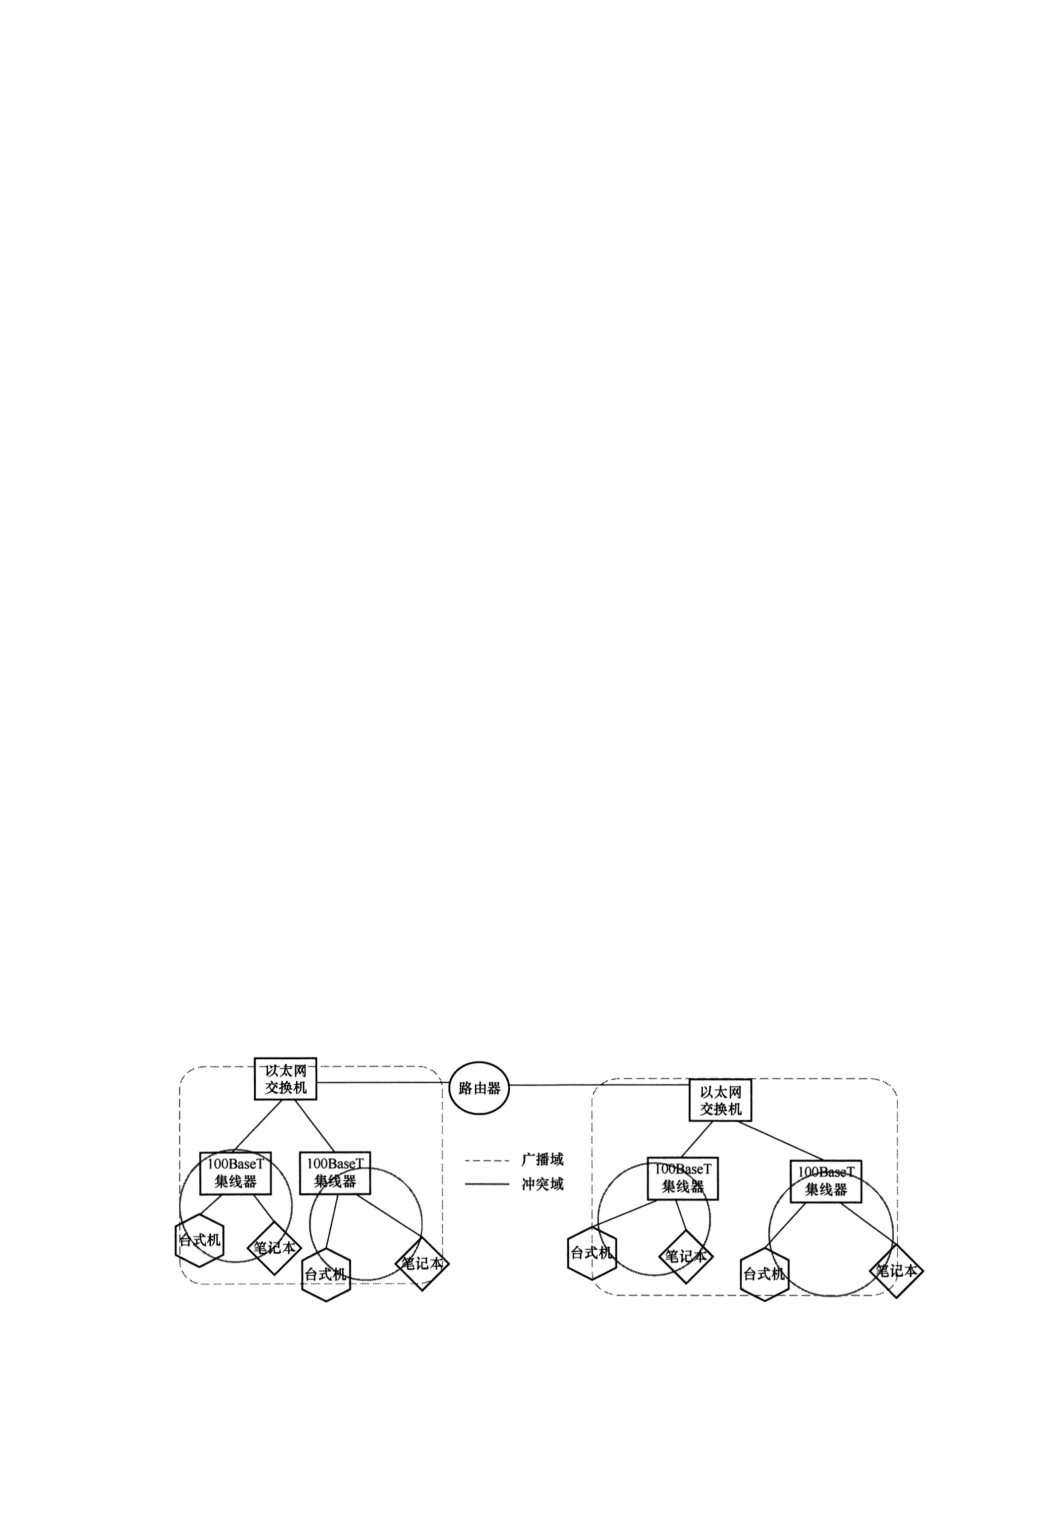
\includegraphics[width=.65\linewidth,height=.4\textheight,keepaspectratio]{../assets/figures/2020-answers-p007-b006.pdf}\end{center}

36. 【解析】发送数据帧和确认帧的时间均为 \(\displaystyle t=1000\times8\mathrm{b}/10\mathrm{kbps}=800\mathrm{ms}\)。


发送周期 \(\displaystyle T=800\mathrm{ms}+200\mathrm{ms}+800\mathrm{ms}+200\mathrm{ms}=2000\mathrm{ms}\)。信道利用率 \(\displaystyle =t/T\times100\%=800/2000\times100\%=40\%\)。


37. 【解析】为了尽量避免碰撞，802.11规定，所有站在完成发送后，必须等待一段很短的时间（继续监听）才能发送下一帧。这段时间称为帧间间隔（InterFrame Space,IFS）。帧间间隔的长短取决于该站要发送的帧的类型。IEEE802.11使用3 种帧间间隔：DIFS（分布式协调 IFS）：最长IFS，优先级最低，用于异步帧竞争访问时延。PIFS（点协调IFS）：中等长度IFS，优先级居中，在 PCF操作中使用。SIFS（短IFS）：最短的IFS，优先级最高，用于需要立即响应的操作。网络中的控制帧及所接收数据的确认帧都采用 SIFS 作为发送之前的等待时延。当结点要发送数据帧时，载波监听到信道空闲时，需等待 DIFS 后发送 RTS 预约信道，图中 IFS1对应的是帧间间隔 DIFS，时间最长，图中IFS2、IFS3、IFS4对应 SIFS。


38. 【解析】由于慢开始门限ssthresh 可以根据需求设置，为了求拥塞窗口从 8KB增长到 32KB 所需的最长时间，可以假定慢开始门限小于等于 8KB，只要不出现拥塞，拥塞窗口就都是加法增大，每经历一个传输轮次（RTT），拥塞窗口逐次加1，所需最长时间为（32-8）\(\displaystyle \times\)2ms=48ms。


39. 【解析】甲与乙建立TCP连接时发送 SYN 段中的序号为1000，则在数据传输阶段所用的起始序号为1001：断开连接时，甲发送给乙 FIN段中的序号为5001，在无任何重传的情况下，甲向乙已经发送应用层数据字节数为5001-1001=4000。


40. 【解析】题中 RTT均为局域网内主机（主机H、本地域名服务器）访问 Internet 上各服务器的往返时间，且忽略其他时延，因此主机H向本地域名服务器的查询时延忽略不计。最短时间：本地主机中有该域名到 IP 地址对应记录，因此不需要 DNS查询时延，直接和www.abc.com 服务器建立TCP 连接再进行资源访问，TCP 连接建立需要1个 RTT，接着发送访问请求并收到服务器资源响应需要1个RTT，共计2个RTT，即 20ms：最长时间：本地主机递归查询本地域名服务器（延时忽略），本地服务器依次迭代查询根域名服务器、com顶级域名服务器、abc.com 域名服务器，共3个 RTT，查询到 IP 地址后，将该映射返回给主机H，主机H和 www.abc.com 服务器建立 TCP 连接再进行资源访问，共2个RTT，因此最长时间需要3+2=5个RTT，即 50ms。


\subsection*{二、综合应用题}

41. 【解析】分析。由 \(\displaystyle D=|a-b|+|b-c|+|c-a|\ge0\) 得：\textcircled{1} 当 \(\displaystyle a=b=c\) 时，距离最小。\textcircled{2} 其余情况。不失一般性，假设 \(\displaystyle a\le b\le c\)，观察下面的数轴：


\begin{center}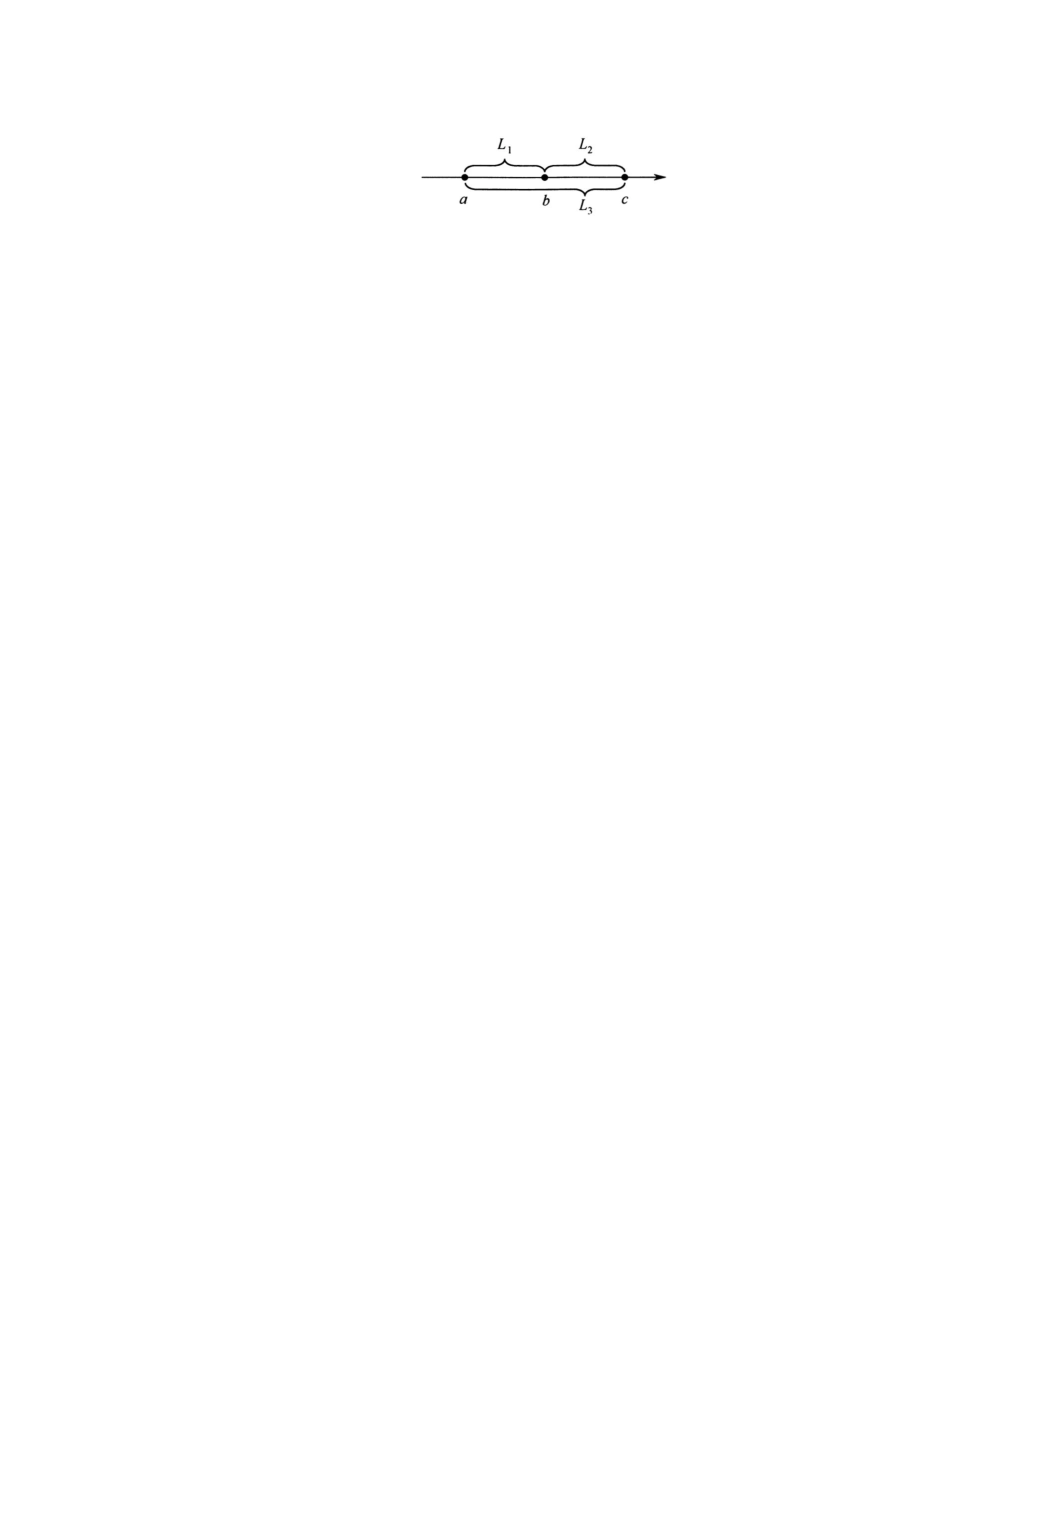
\includegraphics[width=.65\linewidth,height=.4\textheight,keepaspectratio]{../assets/figures/2020-answers-p009-b000.pdf}\end{center}

\(\displaystyle L_1=|a-b|\)，\(\displaystyle L_2=|b-c|\)，\(\displaystyle L_3=|c-a|\)，\(\displaystyle D=|a-b|+|b-c|+|c-a|=L_1+L_2+L_3=2L_3\)。由 \(\displaystyle D\) 的表达式可知，事实上决定 \(\displaystyle D\) 大小的关键是 \(\displaystyle a\) 和 \(\displaystyle c\) 之间的距离，于是问题就可以简化为每次固定 \(\displaystyle c\) 找一个 \(\displaystyle a\) 使得 \(\displaystyle L_3=|c-a|\) 最小。


（1）算法的基本设计思想：\textcircled{1} 使用 \(\displaystyle D_{\displaystyle \min}\) 记录所有已处理过的三元组的最小距离，初值为一个足够大的整数。\textcircled{2} 集合 \(\displaystyle S_1,\allowbreak S_2,\allowbreak S_3\) 分别保存在数组 A、B、C 中。数组的下标变量 \(\displaystyle i=j=k=0\)，当 \(\displaystyle i<|S_1|\)、\(\displaystyle j<|S_2|\) 且 \(\displaystyle k<|S_3|\) 时（\(\displaystyle |S|\) 表示集合 \(\displaystyle S\) 中的元素个数），循环执行 a)～c)。a) 计算 (A[i],B[j],C[k]) 的距离 \(\displaystyle D\)；（计算 \(\displaystyle D\)）b) 若 \(\displaystyle D<D_{\displaystyle \min}\)，则 \(\displaystyle D_{\displaystyle \min}=D\)；（更新 \(\displaystyle D\)）c) 将 A[i]、B[j]、C[k] 中的最小值的下标加 1；（对照分析：最小值为 \(\displaystyle a\)，最大值为 \(\displaystyle c\)，这里 \(\displaystyle c\) 不变而更新 \(\displaystyle a\)，试图寻找更小距离 \(\displaystyle D\)）\textcircled{3} 输出 \(\displaystyle D_{\displaystyle \min}\)，结束。


（2）算法实现：


\begin{Verbatim}[breaklines,breakanywhere,fontsize=\small]
#define INT_MAX 0x7fffffff
int abs_(int a) {                   //计算绝对值
    if(a<0) return -a;
    else return a;
}
bool xIs_min(int a,int b,int c) {  //a是否是三个数中的最小值
    if(a<=b&&a<=c) return true;
    return false;
}
int findMinofTrip(int A[],int n,int B[],int m,int C[],int p) {
    //D_min用于记录三元组最小距离，初值赋为INT_MAX
    int i=0,j=0,k=0,D_min=INT_MAX,D;
    while(i<n&&j<m&&k<p&&D_min>0) {
        D=abs_(A[i]-B[j])+abs_(B[j]-C[k])+abs_(C[k]-A[i]); //计算D
        if(D<D_min) D_min=D;                              //更新D
        if(xIs_min(A[i],B[j],C[k])) i++;                  //更新a
        else if(xIs_min(B[j],C[k],A[i])) j++;
        else k++;
    }
    return D_min;
}
\end{Verbatim}

（3）设 \(\displaystyle n=|S_1|+|S_2|+|S_3|\)，时间复杂度为 \(\displaystyle O(n)\)，空间复杂度为 \(\displaystyle O(1)\)。


42. 【解析】（1）使用一棵二叉树保存字符集中各字符的编码，每个编码对应于从根开始到达某叶结点的一条路径，路径长度等于编码位数，路径到达的叶结点中保存该编码对应的字符。（2）从左至右依次扫描 0/1 串中的各位。从根开始，根据串中当前位沿当前结点的左子指针或右子指针下移，直到移动到叶结点时为止。输出叶结点中保存的字符。然后从根开始重复这个过程，直到扫描到 0/1 串结束，译码完成。


（3）二叉树既可用于保存各字符的编码，又可用于检测编码是否具有前缀特性。判定编码是否具有前缀特性的过程，也是构建二叉树的过程。初始时，二叉树中仅含有根结点，其左子指针和右子指针均为空。依次读入每个编码 C，建立/寻找从根开始对应于该编码的一条路径，过程如下：对每个编码，从左至右扫描 C 的各位，根据 C 当前位（0 或 1）沿结点的指针（左子指针或右子指针）向下移动。当遇到空指针时，创建新结点，让空指针指向该新结点并继续移动。沿指针移动的过程中，可能遇到三种情况：\textcircled{1} 若遇到了叶结点（非根），则表明不具有前缀特性，返回。\textcircled{2} 若在处理 C 的所有位的过程中，均没有创建新结点，则表明不具有前缀特性，返回。\textcircled{3} 若在处理 C 的最后一个编码位时创建了新结点，则继续验证下一个编码。若所有编码均通过验证，则编码具有前缀特性。


43. 【解析】（1）乘法运算可以通过加法和移位来实现。编译器可以将乘法运算转换为一个循环代码段，在循环代码段中通过比较、加法和移位等指令实现乘法运算。（2）控制逻辑的作用是控制循环次数，控制加法和移位操作。（3）\textcircled{1} 最长，\textcircled{3} 最短。对于\textcircled{1}，需要用循环代码段（即软件）实现乘法操作，因而需要反复执行很多条指令，而每条指令都需要取指令、译码、取数、执行并保存结果，所以执行时间很长；对于\textcircled{2}和\textcircled{3}，都只需用一条乘法指令实现乘法操作，不过\textcircled{2}中的乘法指令需要多个时钟周期才能完成，而\textcircled{3}中的乘法指令可以在一个时钟周期内完成，所以\textcircled{3}的执行时间最短。


（4）当 \(\displaystyle n=32,\allowbreak x=2^{31}-1,\allowbreak y=2\) 时，带符号整数和无符号整数乘法指令得到的 64 位乘积都是 0000 0000 FFFF FFFEH。int 型的表示范围为 \(\displaystyle [-2^{31},\allowbreak 2^{31}-1]\)，故函数 imul() 的结果溢出；unsigned int 型的表示范围为 \(\displaystyle [0,\allowbreak 2^{32}-1]\)，故函数 umul() 的结果不溢出。对于无符号整数乘法，若乘积高 \(\displaystyle n\) 位全为 0，即使低 \(\displaystyle n\) 位全为 1 也正好是 \(\displaystyle 2^{32}-1\)，不溢出，否则溢出。


44. 【解析】（1）主存块大小为 \(\displaystyle 64\mathrm{B}=2^6\) 字节，所以主存地址低 6 位为块内地址，Cache 组数为 \(\displaystyle 32\mathrm{KB}/(64\mathrm{B}\times8)=64=2^6\)，故主存地址中间 6 位为 Cache 组号，主存地址中高 \(\displaystyle 32-6-6=20\) 位为标记，采用 8 路组相联映射，故每行中 LRU 位占 3 位，采用直写方式，故没有修改位。


（2）0080 00C0H = 0000 0000 1000 0000 0000 0000 1100 0000B，主存地址低 6 位为块内地址，为全 0，故 s 位于一个主存块的开始处，占 1024\(\displaystyle \times\)4B/64B = 64 个主存块；在执行程序段的过程中，每个主存块中的 64B/4B = 16 个数组元素依次读、写 1 次，因而对每个主存块，总是第一次访问缺失，此时会将整个主存块调入 Cache，之后每次都命中。综上，数组 s 的数据 Cache 访问缺失次数为 64 次。


（3）0001 0003H = 0000 0000 0000 0001 0000 0000 0000 0011B，根据主存地址划分可知，组索引为 0，故该地址所在主存块映射到指令 Cache 的第 0 组；因为 Cache 初始为空，所有 Cache 行的有效位均为 0，所以 Cache 访问缺失。此时，将该主存块取出后存入指令 Cache 的第 0 组的任意一行，并将主存地址高 20 位（00010H）填入该行标记字段，设置有效位，修改 LRU 位，最后根据块内地址 000011B 从该行中取出相应内容。


45. 【解析】本题要求实现操作的先后顺序，没有互斥关系，是一个简单的同步问题。本题虽然有 5 个操作，但是只有 4 个同步关系，因此分别设置信号量 SAC、SBC、SCE 和 SDE 对应 4 个同步关系。


\begin{Verbatim}[breaklines,breakanywhere,fontsize=\small]
Semaphore SAC = 0;     //控制A和C的执行顺序
Semaphore SBC = 0;     //控制B和C的执行顺序
Semaphore SCE = 0;     //控制C和E的执行顺序
Semaphore SDE = 0;     //控制D和E的执行顺序
\end{Verbatim}

5 个操作可描述为如下：


\begin{Verbatim}[breaklines,breakanywhere,fontsize=\small]
CoBegin
A() {
    完成动作A;
    V(SAC);              //实现A、C之间的同步关系
}
B() {
    完成动作B;
    V(SBC);              //实现B、C之间的同步关系
}
C() {
    //C必须在A、B都完成后才能完成
    P(SAC);
    P(SBC);
    完成动作C;
    V(SCE);              //实现C、E之间的同步关系
}
D() {
    完成动作D;
    V(SDE);              //实现D、E之间的同步关系
}
E() {
    //E必须在完成C、D之后执行
    P(SCE);
    P(SDE);
    完成动作E;
}
CoEnd
\end{Verbatim}

46. 【解析】（1）\textcircled{1} 页面大小 \(\displaystyle =2^{12}\mathrm{B}=4096\mathrm{B}=4\mathrm{KB}\)。每个数组元素 4B，每个页面可以存放 4KB/4B = 1024 个数组元素，正好是数组的一行，数组 a 按行优先方式存放。1080 0000H 的虚页号为 10800H，因此 a[0] 行存放在虚页号为 10800H 的页面中，a[1] 行存放在页号为 10801H 的页面中。a[1][2] 的虚拟地址为 10801 000H + 4\(\displaystyle \times\)2 = 10801 008H。\textcircled{2} 转换为二进制 0001 0000 1000 0000 0000 0001 0000 0000 1000，根据虚拟地址结构可知，对应的页目录号为 042H，页号为 001H。\textcircled{3} 进程的页目录表起始地址为 0020 1000H，每个页目录项长 4B，因此 042H 号页目录项的物理地址是 0020 1000H + 4\(\displaystyle \times\)42H = 0020 1108H。\textcircled{4} 页目录项存放的页框号为 00301H，二级页表的起始地址为 00301 000H，因此 a[1][2] 所在页的页号为 001H，每个页表项 4B，因此对应的页表项物理地址是 00301 000H + 001H\(\displaystyle \times\)4 = 00301 004H。


（2）根据数组随机存取的特点，数组 a 在虚拟地址空间中所占的区域必须连续，由于数组 a 不止占用一页，相邻逻辑页在物理上不一定相邻，因此数组 a 在物理地址空间中所占的区域可以不连续。（3）由（1）可知每个页面正好可以存放一整行的数组元素，“按行优先方式存放”意味着数组的同一行的所有元素都存放在同一个页面中，同一列的各个元素都存放在不同的页面中，因此数组 a 按行遍历的局部性较好。


47. 【解析】（1）两个子网使用了相同的网段，且路由器开启了 NAT 功能，加上题干给出了 NAT 表的结构，因此需要配置 NAT 表。路由器 R2 开启 NAT 服务，当路由器 R2 从 WAN 口收到 H2 或 H3 发来的数据时，根据 NAT 表发送给 Web 服务器的对应端口。外网 IP 地址应该为该路由器的外端 IP 地址，内网 IP 地址应该为 Web 服务器的地址，Web 服务器的默认端口为 80，因此内网端口号固定为 80，当其他网络的主机访问 Web 服务器时，默认访问的端口应该也是 80，但是访问的目的 IP 是路由器的 IP 地址，因此 NAT 表中的外部端口最好也统一为 80。题目中并未要求对 H1 进行访问，因此 H1 的 NAT 表项可以不写。R2 的 NAT 表配置如下：


\begin{center}\begin{adjustbox}{max width=\linewidth}\begin{tabular}{|>{\raggedright\arraybackslash}p{\dimexpr(\linewidth-8\tabcolsep-5\arrayrulewidth)/4\relax}|>{\raggedright\arraybackslash}p{\dimexpr(\linewidth-8\tabcolsep-5\arrayrulewidth)/4\relax}|>{\raggedright\arraybackslash}p{\dimexpr(\linewidth-8\tabcolsep-5\arrayrulewidth)/4\relax}|>{\raggedright\arraybackslash}p{\dimexpr(\linewidth-8\tabcolsep-5\arrayrulewidth)/4\relax}|}\hline
外网 IP 地址 & 外网端口号 & 内网 IP 地址 & 内网端口号\\\hline
203.\allowbreak{}10.\allowbreak{}2.\allowbreak{}2 & 80 & 192.\allowbreak{}168.\allowbreak{}1.\allowbreak{}2 & 80\\\hline\end{tabular}\end{adjustbox}\end{center}

（2）由于启用了 NAT 服务，H2 发送的 P 的源 IP 地址应该是 H2 的内网地址，目的地址应该是 R2 的外网 IP 地址，源 IP 地址是 192.168.1.2，目的 IP 地址是 203.10.2.2。R3 转发后，将 P 的源 IP 地址改为 R3 的外网 IP 地址，目的 IP 地址仍然不变，源 IP 地址是 203.10.2.6，目的 IP 地址是 203.10.2.2。R2 转发后，将 P 的目的 IP 地址改为 Web 服务器的内网地址，源地址仍然不变，源 IP 地址是 203.10.2.6，目的 IP 地址是 192.168.1.2。


\subsection*{2019 全国硕士研究生招生考试计算机学科专业基础试题}

\subsection*{一、单项选择题}

第 01～40 小题，每小题 2 分，共 80 分。下列每题给出的四个选项中，只有一个选项最符合试题要求。


01. 设 \(\displaystyle n\) 是描述问题规模的非负整数，下列程序段的时间复杂度是（　）。


\begin{Verbatim}[breaklines,breakanywhere,fontsize=\small]
x=0;
while (n>=(x+1)*(x+1))
    x=x+1;
\end{Verbatim}

A. \(\displaystyle O(\log n)\)　B. \(\displaystyle O(n^{1/2})\)　C. \(\displaystyle O(n)\)　D. \(\displaystyle O(n^2)\)


02. 若将一棵树 T 转化为对应的二叉树 BT，则下列对 BT 的遍历中，其遍历序列与 T 的后根遍历序列相同的是（　）。A. 先序遍历　B. 中序遍历　C. 后序遍历　D. 按层遍历


03. 对 n 个互不相同的符号进行哈夫曼编码。若生成的哈夫曼树共有 115 个结点，则 n 的值是（　）。A. 56　B. 57　C. 58　D. 60


04. 在任意一棵非空平衡二叉树（AVL 树）\(\displaystyle T_1\) 中，删除某结点 v 之后形成平衡二叉树 \(\displaystyle T_2\)，再将 v 插入 \(\displaystyle T_2\) 形成平衡二叉树 \(\displaystyle T_3\)。下列关于 \(\displaystyle T_1\) 与 \(\displaystyle T_3\) 的叙述中，正确的是（　）。\(\displaystyle \mathrm{I}\). 若 v 是 \(\displaystyle T_1\) 的叶结点，则 \(\displaystyle T_1\) 与 \(\displaystyle T_3\) 可能不相同。\(\displaystyle \mathrm{II}\). 若 v 不是 \(\displaystyle T_1\) 的叶结点，则 \(\displaystyle T_1\) 与 \(\displaystyle T_3\) 一定不相同。\(\displaystyle \mathrm{III}\). 若 v 不是 \(\displaystyle T_1\) 的叶结点，则 \(\displaystyle T_1\) 与 \(\displaystyle T_3\) 一定相同。A. 仅\(\displaystyle \mathrm{I}\)　B. 仅\(\displaystyle \mathrm{II}\)　C. 仅\(\displaystyle \mathrm{I}\)、\(\displaystyle \mathrm{II}\)　D. 仅\(\displaystyle \mathrm{I}\)、\(\displaystyle \mathrm{III}\)


05. 下图所示的 AOE 网表示一项包含 8 个活动的工程。活动 d 的最早开始时间和最迟开始时间分别是（　）。


\begin{center}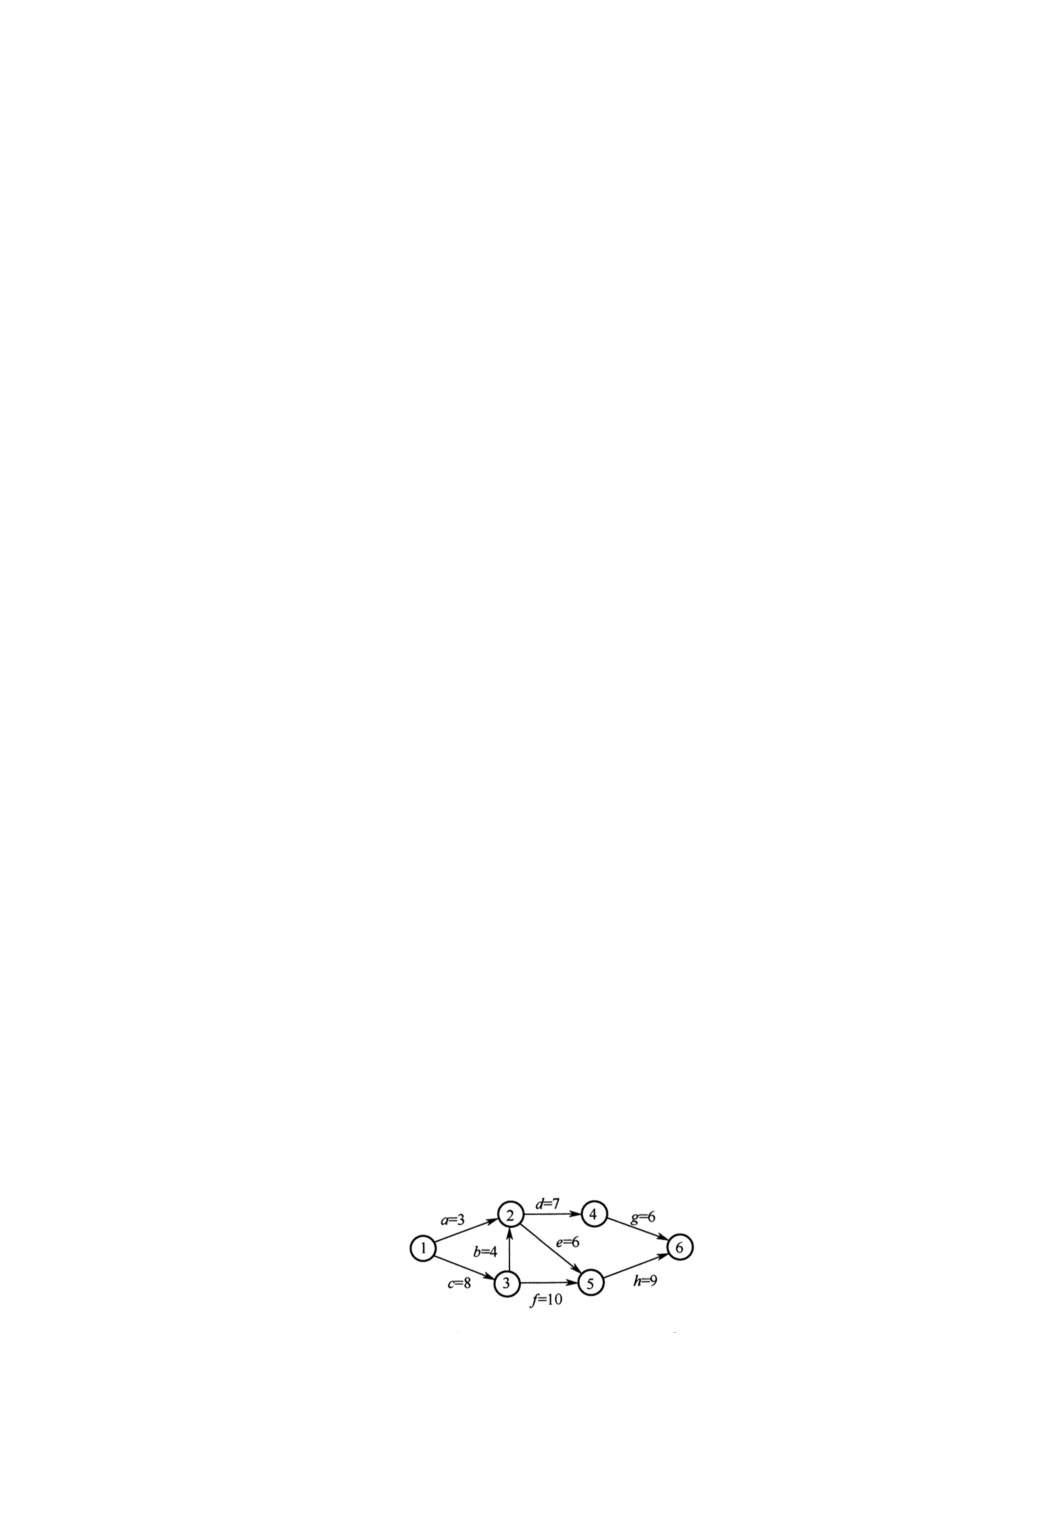
\includegraphics[width=.65\linewidth,height=.4\textheight,keepaspectratio]{../assets/figures/2020-answers-p013-b010.pdf}\end{center}

A. 3 和 7　B. 12 和 12　C. 12 和 14　D. 15 和 15


06. 用有向无环图描述表达式 \(\displaystyle (x+y)((x+y)/x)\)，需要的顶点个数至少是（　）。

\end{document}
